\documentclass{exam}

\usepackage[dvipsnames]{xcolor}
\usepackage{amsmath}
\usepackage{amsfonts}
\usepackage{amsthm}
\usepackage{microtype}
\usepackage{siunitx}
\DeclareSIUnit\year{yr}
\usepackage{pgfplots}
\usepackage{graphicx}
\usepackage{sidecap}
\sidecaptionvpos{figure}{c}
\usepackage{float}
\usepackage{gensymb}
\usepackage{tkz-euclide}
\usetkzobj{all}
\usepackage{commath}
\usepackage[version=4]{mhchem}

\newtheorem*{thm}{Theorem}


% russian integral
\usepackage{scalerel}
\DeclareMathOperator*{\rint}{\scalerel*{\rotatebox{17}{$\!\int\!$}}{\int}}

% \qformat{Question \thequestion: \thequestiontitle\hfill}

\begin{document}
\begin{questions}

\section*{NCEA Level 1 Mathematics (Trigonometry)}

\question A person \SI{100}{\metre} from the base of a tree estimates that the angle  between his eye level (around \SI{1.5}{\metre} above
          the ground) and the top of the tree is \SI{18}{\degree}. Compute the height of the tree.
\question The angle of elevation of a balloon moving straight up changes from \SI{25}{\degree} at 10:00 am to \SI{60}{\degree} at 10:02 am. The point
          of observation of the angle of elevation is situated \SI{200}{\metre} away from the take off point. If the balloon is moving upwards at a
          constant speed $ v $, compute $ v $ to a reasonable accuracy.
\question Consider the diagram below.
          \begin{center}
            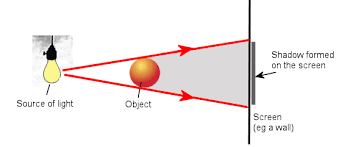
\includegraphics[width=0.5\textwidth]{shadow1}
          \end{center}
          The radius of the ball is sixteen centimetres, the distance from the screen to the light source is two metres, and
          the centre of the ball is exactly halfway between the light source and the screen, find the height of the shadow formed.
\question Prove that $ \sin \theta = \cos(\SI{90}{\degree} -  \theta) $.
\question Show that $ \sin \SI{45}{\degree} = \frac{1}{\sqrt{2}} $ exactly.
\question Suppose a triangle has two sides, measuring \SI{4}{\metre} and \SI{5}{\metre} respectively. If the angle between these sides
          is \SI{40}{\degree}, what is the angle of the triangle?
\question Consider a circle, along with a ray $ AC $ from the centre and tangents $ BF $ and $ CE $. Show that $ \ell(CE) = \ell(BF) = \tan \alpha $.
          \begin{center}
            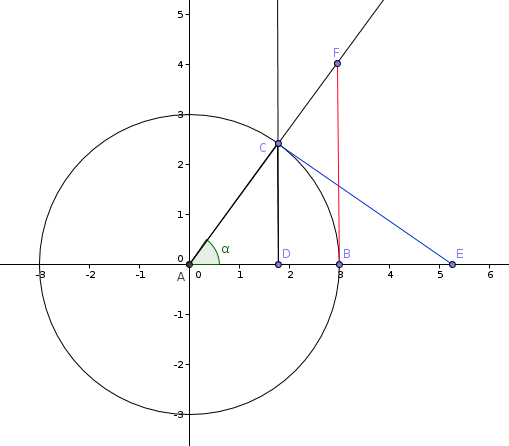
\includegraphics[width=0.5\textwidth]{wowtrig}
          \end{center}
\question A \textbf{regular $n$-gon} ($ n \geq 3 $) is a shape with exactly $ n $ sides, each with exactly the same length. For example,
          a regular 3-gon is an equilateral triangle. Find the internal angle between the sides of (a) a regular 3-gon, (b) a regular 4-gon,
          and (c) a regular $n$-gon (for $ n $ any natural number).
\question In Ye Olden Days(TM), long distances were measured and maps drawn using triangulation. Consider the following map, where each
          point $ A $, $ B $, $ C $, and  $ D $ is a mountain,
          \begin{center}
            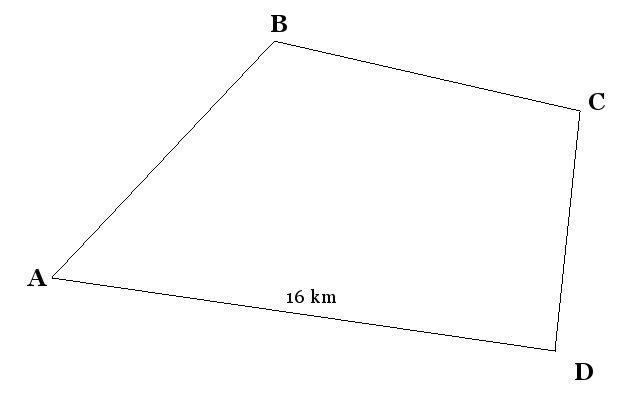
\includegraphics[width=0.5\textwidth]{survey}
          \end{center}
          The distance $ \ell(AD) $ is known to be \SI{16}{\kilo\metre}, and the angles $ \angle BAD $, $ \angle ABC $, and $ \angle ADC $ are measured
          to be \SI{30}{\degree}, \SI{110}{\degree}, and \SI{100}{\degree} respectively. In terms of height, $ D $ is measured to be \SI{10}{\degree}
          below $ A $ and $ C $ is measured to be \SI{14}{\degree} above $ D $. The height of peak $ A $ is \SI{1100}{\metre}. What is the straight-line
          distance between the tops of peaks $ A $ and $ D $, and what is the height of the peak at $ D $? Is it possible to calculate the height
          of peak $ B $?
\question Take a regular tetrahedron (triangular pyramid) and drop a perpendicular line from the incentre of each face; at the point in the
          centre of the solid where the three lines meet, what angle does each line form with the others?
\question You know that for a right-angled triangle, the Pythagorean Theorem can be used to calculate the length of any side given the
          other two. In this question, we will derive a more general side-length formula that works for arbitrary triangles.
          
          Let us consider an arbitrary triangle $ ABC $, and move it around so that the point $ C $ is at $ (0,0) $ and the point $ B $ is at $ (b, 0) $;
          see the following diagram.
          \begin{center}
            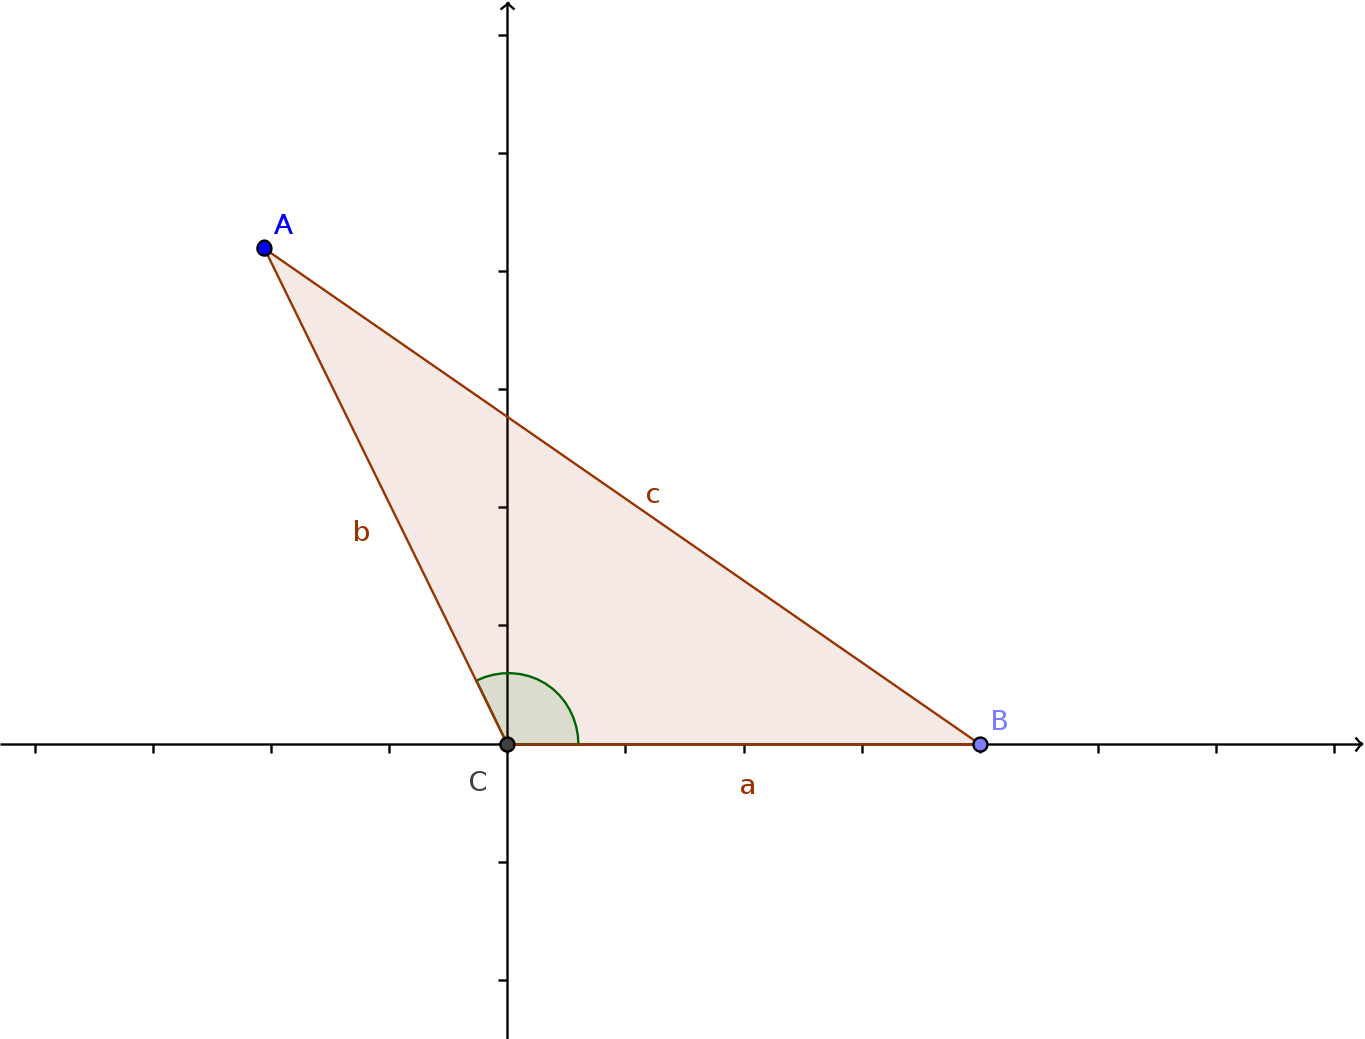
\includegraphics[width=0.5\textwidth]{cosinerule1}
          \end{center}
  \begin{parts}
    \part Let $ \theta $ be the measure of the angle $ \angle ACB $. Show that the coordinates of the point $ A $ are $ (b\cos\theta, b\sin\theta) $.
    \part Use the Pythagorean Theorem to calculate the distance $ c $ using the coordinates of $ A $ and $ B $.
    \part Hence show that
      \begin{equation}
        c^2 = a^2 + b^2 - 2ab\cos \theta. \tag{Cosine rule.}
      \end{equation}
  \end{parts}
\question Calculate the bond angle of a methane molecule (\ce{CH4}).
\end{questions}
\end{document}
